%!TEX root = ../NeuralNets.tex
\section{Activation Functions}\label{sec:activation-functions}\xindex{activation functions}%

\subsection{Step Function}
\begin{equation}\label{eq:step_function}
\phi(x) =
	\begin{cases}
		1 & \text{if}\, x > 0\\
		0 & \text{if}\, x \leq 0
	\end{cases}
\end{equation}
The derivative is always 0.
\begin{figure}
\centering
\begin{tikzpicture}
\begin{axis}[
	axis lines = middle,
	xlabel = $x$,
	ylabel = $y$,
	ymin = -0.5,
	ymax = 1.5,
	xmin = -1,
	xmax = 1,
	clip = false,
]
\addplot[
	color = blue,
	thick
] coordinates {(-1,0)(0,0)(0,1)(1,1)}
node[above,pos=1] {$\phi(x)$};
\end{axis}
\end{tikzpicture}
\caption{Step Function}
\end{figure}

\subsection{Sigmoid}\label{sec:sigmoid}
Most common activation function, can saturate and is easy to deviate.
\begin{equation}\label{ed:sigmoid}
\sigma(x) = \frac{1}{1 + e^{-\beta x}}
\end{equation}
And it's derivative:
\begin{align}\label{ed:sigmoid_derivative}
\begin{split}
\frac{d\,\sigma(x)}{d\,x} &= \frac{d}{d\,x} (1 + e^{-\beta x})^{-1}\\
&= (-1) (1 + e^{-\beta x})^{-2} (-\beta e^{-\beta x})\\
&= \beta (1 + e^{-\beta x})^{-2} e^{-\beta x}\\
&= \beta \frac{1}{1 + e^{-\beta x}} \frac{e^{-\beta x}}{1 + e^{-\beta x}}\\
&= \beta \sigma(x) \frac{e^{-\beta x} + 1 - 1}{1 + e^{-\beta x}}\\
&= \beta \sigma(x) (1 - \frac{1}{1 + e^{-\beta x}})\\
&= \beta \sigma(x) (1 - \sigma(x))
\end{split}
\end{align}
And because there exists algorithm using this, you should have seen the second derivative as well ($\beta=1$):
\begin{align}
\begin{split}
\frac{d\,\sigma(x)(1-\sigma(x))}{d\,x} &= (1-\sigma(x)) \frac{d\,\sigma(x)}{d\,x} + \sigma(x) \frac{d\,(1-\sigma(x))}{d\,x}\\
&= (1-\sigma(x)) \sigma(x) (1 - \sigma(x)) + \sigma(x) (-1) \sigma(x) (1 - \sigma(x))\\
&= \sigma(x) (1 - \sigma(x))^2 - \sigma(x)^2 (1 - \sigma(x))
\end{split}
\end{align}

\begin{figure}
\centering
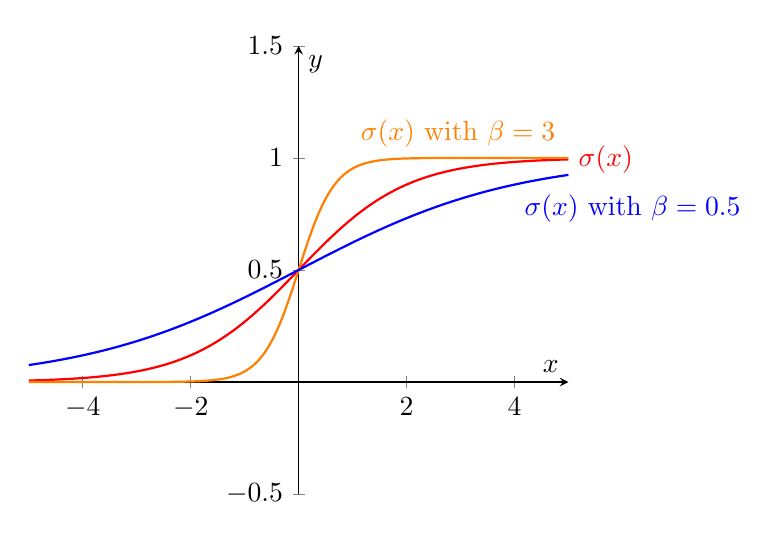
\begin{tikzpicture}
\begin{axis}[
	axis lines = middle,
	xlabel = $x$,
	ylabel = $y$,
	ymin = -0.5,
	ymax = 1.5,
	xmin = -5,
	xmax = 5,
	clip = false,
]
\addplot[
	samples = 100,
	color = red,
	thick, smooth,
	]
{1/(1+e^(-x))}
node[right,pos=1] {$\sigma(x)$};
\addplot[
	samples = 100,
	color = orange,
	thick, smooth,
	]
{1/(1+e^(-3*x))}
node[above,pos=0.8] {$\sigma(x)$ with $\beta=3$};
\addplot[
	samples = 100,
	color = blue,
	thick, smooth,
	]
{1/(1+e^(-0.5*x))}
node[below right,pos=0.9] {$\sigma(x)$ with $\beta=0.5$};
\end{axis}
\end{tikzpicture}
\caption{Sigmoid function with $\beta=1$ (red), $\beta=3$ (orange) and $\beta=0.5$ (blue).}
\end{figure}

\begin{figure}
\centering
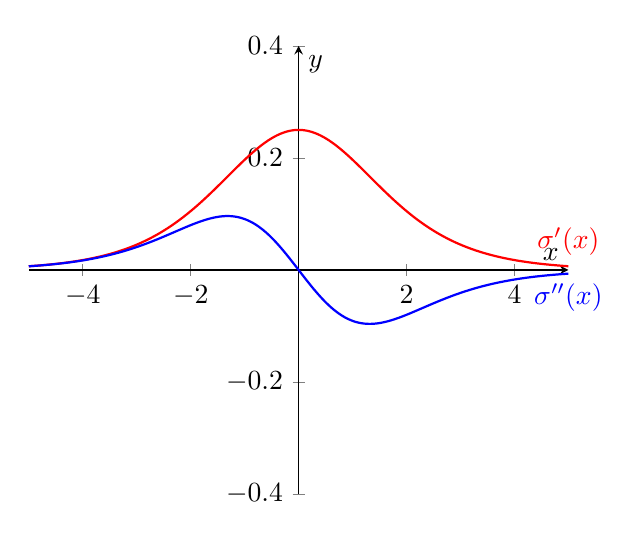
\begin{tikzpicture}
\begin{axis}[
	axis lines = middle,
	xlabel = $x$,
	ylabel = $y$,
	ymin = -0.4,
	ymax = 0.4,
	xmin = -5,
	xmax = 5,
	clip = false,
]
\addplot[
	samples = 100,
	color = red,
	thick, smooth,
	]
{(1/(1+e^(-x)))*(1-(1/(1+e^(-x))))}
node[above,pos=1] {$\sigma'(x)$};
\addplot[
	samples = 100,
	color = blue,
	thick, smooth,
	]
{(1/(1+e^(-x)))*(1-(1/(1+e^(-x))))^2 - (1/(1+e^(-x)))^2*(1-(1/(1+e^(-x))))}
node[below,pos=1] {$\sigma''(x)$};
\end{axis}
\end{tikzpicture}
\caption{First and second derivative of the sigmoid function.}
\end{figure}

\subsection{Softmax Function}
In a classification problem we would like $\mathbf{a}$ to be a probability distribution ($\Rightarrow \sum_i a_i = 1$). The softmax function will output a posteriori probability ($p(k|x$) and the biggest value from the layer below is very likely to be close to $1$.
\begin{equation}\label{ed:softmax}
a_i = \phi(z_i) = \frac{e^{z_i}}{\sum_j e^{z_j}}
\end{equation}
And it's derivative:
\begin{align}
\begin{split}\label{ed:softmax_derivative}
\frac{\partial \phi(z_i)}{\partial z_i}
&= \frac{\left(\frac{\partial}{\partial z_i} e^{z_i}\right)(\sum_j e^{z_j}) - e^{z_i} \left(\frac{\partial}{\partial z_i}(\sum_j e^{z_j})\right)}{(\sum_j e^{y_j})^2}\\
&= \frac{e^{y_i} \sum_j e^{y_j} - e^{y_i} e^{y_i}}{(\sum_j e^{y_j})^2}\\
&= \frac{e^{y_i} \sum_j e^{y_j}}{(\sum_j e^{y_j})^2} - \frac{e^{y_i} e^{y_i}}{(\sum_j e^{y_j})^2}\\
&= \frac{e^{y_i}}{\sum_j e^{y_j}} - \left(\frac{e^{y_i}}{\sum_j e^{y_j}}\right)^2\\
&= \phi(y_i) - \phi(y_i)^2\\
&= \phi(y_i) (1 - \phi(y_i))
\end{split}
\end{align}

\subsection{Hyperbolic Tangent Function}
Similar to Sigmoid function, but with outputs in $[-1,1]$. Also not that if the input has a mean of $0$ then so will the output.

\todo{Why is $\tanh$ worth the computational overhead over sigmoid?}
\begin{equation}
\phi(x) = \tanh(x) = \frac{e^x - e^{-x}}{e^x + e^{-x}}
\end{equation}
And it's derivative:
\begin{equation}
\frac{\diff \phi(x)}{\diff x} = 1 - \tanh(x) = \frac{(e^x - e^{-x})^2}{(e^x + e^{-x})^2}
\end{equation}
\begin{figure}
\centering
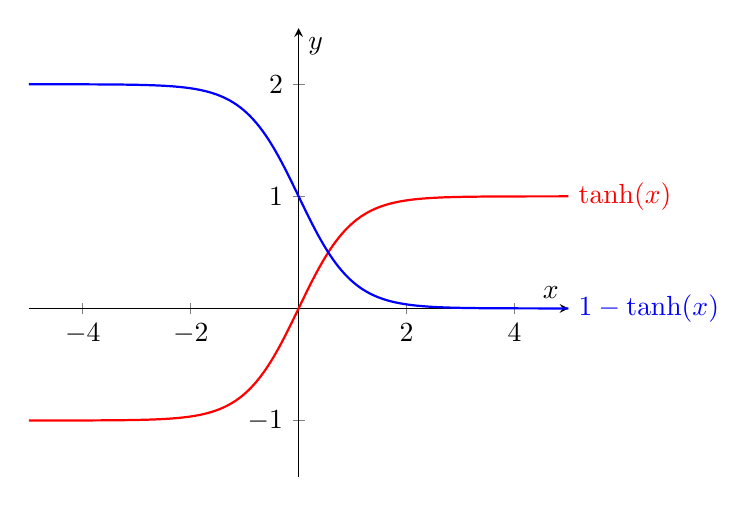
\begin{tikzpicture}
\begin{axis}[
	axis lines = middle,
	xlabel = $x$,
	ylabel = $y$,
	ymin = -1.5,
	ymax = 2.5,
	xmin = -5,
	xmax = 5,
	clip = false,
]
\addplot[
	samples = 100,
	color = red,
	thick, smooth,
	]
{tanh(x)}
node[right,pos=1] {$\tanh(x)$};
\addplot[
	samples = 100,
	color = blue,
	thick, smooth,
	]
{1-tanh(x)}
node[right,pos=1] {$1 - \tanh(x)$};
\end{axis}
\end{tikzpicture}
\caption{Hyperbolic Tangent Function (red) and its derivative (blue).}
\end{figure}

\subsection{Linear Function}
Very simple, but with two big downsides. The gradient is always $1$ and multi-layers using it effectively only do a linear combination and therefore can be left out.
$$\phi(x) = x$$

\begin{figure}
\centering
\begin{tikzpicture}
\begin{axis}[
	axis lines = middle,
	xlabel = $x$,
	ylabel = $y$,
	ymin = -5,
	ymax = 5,
	xmin = -5,
	xmax = 5,
	clip = false,
]
\addplot[
	domain = -5:5,
	samples = 100,
	color = blue,
	thick, smooth,
	]
{x}
node[left,pos=0] {$x$};
\addplot[
	domain = -5:5,
	samples = 100,
	color = red,
	thick, smooth,
	]
{max(0,x)}
node[left,pos=0] {$\max(0,x)$};
\addplot[
	domain = -5:5,
	samples = 100,
	color = orange,
	thick, smooth,
	]
{ln(1+e^x)}
node[right,pos=1] {$\ln(1+e^x)$};
\end{axis}
\end{tikzpicture}
\caption{Linear Function (blue), Rectified Linear Unit (red), Softplus (orange)}
\end{figure}

\subsection{Rectified Linear Unit}
The Rectified Linear Unit (ReLU) is more biologically plausible.
\begin{align}
\phi(x) = \max(0, x)
\intertext{And it's derivative}
\frac{\diff \phi(x)}{\diff x} =
	\begin{cases}
		1 & \text{if}\, x > 0\\
		0 & \text{if}\, x \leq 0\\
	\end{cases}
\end{align}

\subsection{Softplus}
Smoothed version of ReLU.
\begin{align}\label{eq:softplus}
\phi(x) = \ln(1 + e^x)
\intertext{And it's derivative}
\frac{\diff \phi(x)}{\diff x} = \frac{e^x}{1 + e^x} = \frac{1}{e^{-x} + 1}
\end{align}

\subsection{Maxout}
Literature: \cite{Goodfellow2013}

Outputs the maximum of its inputs
\begin{equation}
a_j^{(l)} = \max_i z_i^{(l)}, \quad (j-1)g +1 \leq i \leq j g \\
\end{equation}
where $z_i^{(l)} = b^{(l)} + \sum_k w_{ki}^{(l)} x_k^{(l-1)}$ is the summed input and $g$ the size of the group on which we take the maximum.
